\documentclass[journal]{IEEEtran}

% Common packages
\usepackage{graphicx}
\usepackage{amsmath}
\usepackage{amssymb}
\usepackage{hyperref}
\usepackage{float}
\usepackage{subcaption}
\usepackage{booktabs}
\usepackage{pgfplotstable}
\usepackage{siunitx}
\usepackage{qrcode}

\pgfplotsset{compat=1.18}
\pgfplotstableset{
    col sep=comma,
    every head row/.style={before row=\toprule, after row=\midrule},
    every last row/.style={after row=\bottomrule},
}

\begin{document}

% ---------- TITLE & AUTHOR ----------
\title{ATOMIC SPECTRA and DETERMINATION of RYDBERG'S CONSTANT}
\author{IBRAHIM H.I. ABUSHAWISH \\
Istanbul University, Department of Physics \\
Experiment Date: September 21, 2026, Report Submission Date: \\
Course \& Section Number: PHYS4704}

\markboth{Physics Laboratory Reports}{2026} 

\maketitle

% ---------- ABSTRACT ----------
\begin{abstract}
The objective of this experiment is to investigate the relationship between atomic spectra and the energy levels of atoms, and to determine the Rydberg constant using the Balmer series of hydrogen. The wavelengths of the hydrogen spectral lines ($H_\alpha$, $H_\beta$, $H_\gamma$) were measured using a diffraction grating. The experimental Rydberg constant was calculated from the measured wavelengths and compared with the theoretical value, demonstrating the quantized nature of atomic energy levels.
\end{abstract}

% ---------- INTRODUCTION ----------
\section{Introduction}
With the help of radiation emitted and absorbed by atoms, it is possible to learn about their structure. The Bohr Atomic Model postulates that an electron can only travel in circular orbits whose angular momentum is an integer multiple of $\hbar$. An electron emits or absorbs electromagnetic waves as it passes from one orbit to another. A hydrogen atom can exist in any one of certain energy states for a very short time. Only if the hydrogen atom passes from one fixed state to another does it emit or absorb radiation with an energy equal to the difference between the energies of these two states. This spontaneous emission is the basis of atomic spectra. 

% ---------- THEORY ----------
\section{Theory}
The energy of any steady state of the hydrogen atom is given by the expression:
\begin{equation}
    E_n = -\frac{1}{8} \frac{e^4 m_e}{\varepsilon_0^2 h^2} \frac{1}{n^2} \quad \text{for } n = 1,2,3 \dots
\end{equation}
where $n$ is the Principal Quantum Number. The wavelength $\lambda$ of the spectral transition can be calculated as follows:
\begin{equation}
    E_{n_2} - E_{n_1} = h \nu = \frac{hc}{\lambda}
\end{equation}
\begin{equation}
    \frac{1}{\lambda} = R_{th} \left( \frac{1}{n_1^2} - \frac{1}{n_2^2} \right)
    \label{eq:rydberg}
\end{equation}
where $R_{th}$ is the theoretical Rydberg Constant ($1.097 \times 10^7 \, \mathrm{m^{-1}}$).
When light of wavelength $\lambda$ is incident on a grating with a grating constant $g$, it diffracts. For first-order diffraction ($m=1$), the maximum intensity condition is met when:
\begin{equation}
    \lambda = g \frac{l}{\sqrt{d^2 + l^2}}
    \label{eq:wavelength}
\end{equation}
where $d$ is the distance between the grating and the ruler, and $2l$ is the distance between the same colors on either side of the central maximum. In this experiment, $g = \SI{1.671}{\mu m}$.

% ---------- EXPERIMENTAL SETUP ----------
\section{Experimental Setup}
The experimental setup used in this experiment consists of:
\begin{itemize}
    \item Diffraction Grating
    \item Hydrogen lamp 
    \item Power Supply
    \item Ruler and Screen
\end{itemize}

% ---------- PROCEDURE ----------
\section{Experimental Procedure}
1. Observe the colors on the ruler from the diffracted light. \\
2. For each color, identify the same colors on the ruler on either side of the central maximum and determine the distance $l$ from the center. \\
3. Measure the distance $d$ between the grating and the ruler. \\
4. Calculate the wavelength of the colors using Equation~\ref{eq:wavelength}. \\
5. Determine the principal quantum numbers $n_1$ and $n_2$ for the $H_\alpha$, $H_\beta$, and $H_\gamma$ lines. \\
6. Calculate the experimental Rydberg constant using Equation~\ref{eq:rydberg} and compare with the literature values.

% ---------- DATA ANALYSIS ----------
\section{Data Analysis}
The distance between the grating and the ruler was measured to be $d = \SI{430}{\mm}$. The central maximum position on the ruler was located at $\SI{560}{\mm}$. The positions of the first-order diffraction maxima for the hydrogen spectral lines were observed at $\SI{740}{\mm}$ for the red line ($H_\alpha$), $\SI{730}{\mm}$ for the green/cyan line ($H_\beta$), and $\SI{700}{\mm}$ for the blue/violet line ($H_\gamma$). The distance $l$ from the central maximum was computed by taking the absolute difference. The experimental wavelengths were then computed using Equation~\ref{eq:wavelength} with $g = \SI{1671}{\nm}$. The Rydberg constant $R_{\text{exp}}$ was derived for each line using Equation~\ref{eq:rydberg}. 

% ---------- RESULTS ----------
\section{Results}

\subsection{Data Tables}
The calculated experimental wavelengths $\lambda_{\text{exp}}$ and Rydberg constants $R_{\text{exp}}$ are presented in Table~\ref{tab:results}.

\begin{table}[H]
    \centering
    \caption{Hydrogen Balmer Series Results}
    \label{tab:results}
    \pgfplotstabletypeset[
        columns/Line/.style={string type, column name=\textbf{Line}},
        columns/2l/.style={column name=\textbf{2l (m)}},
        columns/n1/.style={column name=$\mathbf{n_1}$},
        columns/n2/.style={column name=$\mathbf{n_2}$},
        columns/lambdaExp/.style={column name=$\mathbf{\lambda_{exp}}$ \textbf{(nm)}},
        columns/lambdaLit/.style={column name=$\mathbf{\lambda_{lit}}$ \textbf{(nm)}},
        columns/Rexp/.style={string type, column name=$\mathbf{R_{exp}}$ $\mathbf{(m^{-1})}$}
    ]{../report/tables/table1.csv}
\end{table}

\subsection{Graphs}
A visual comparison of the experimental wavelengths against the theoretical literature values is shown in Figure~\ref{fig:wavelength}.

\begin{figure}[H]
    \centering
    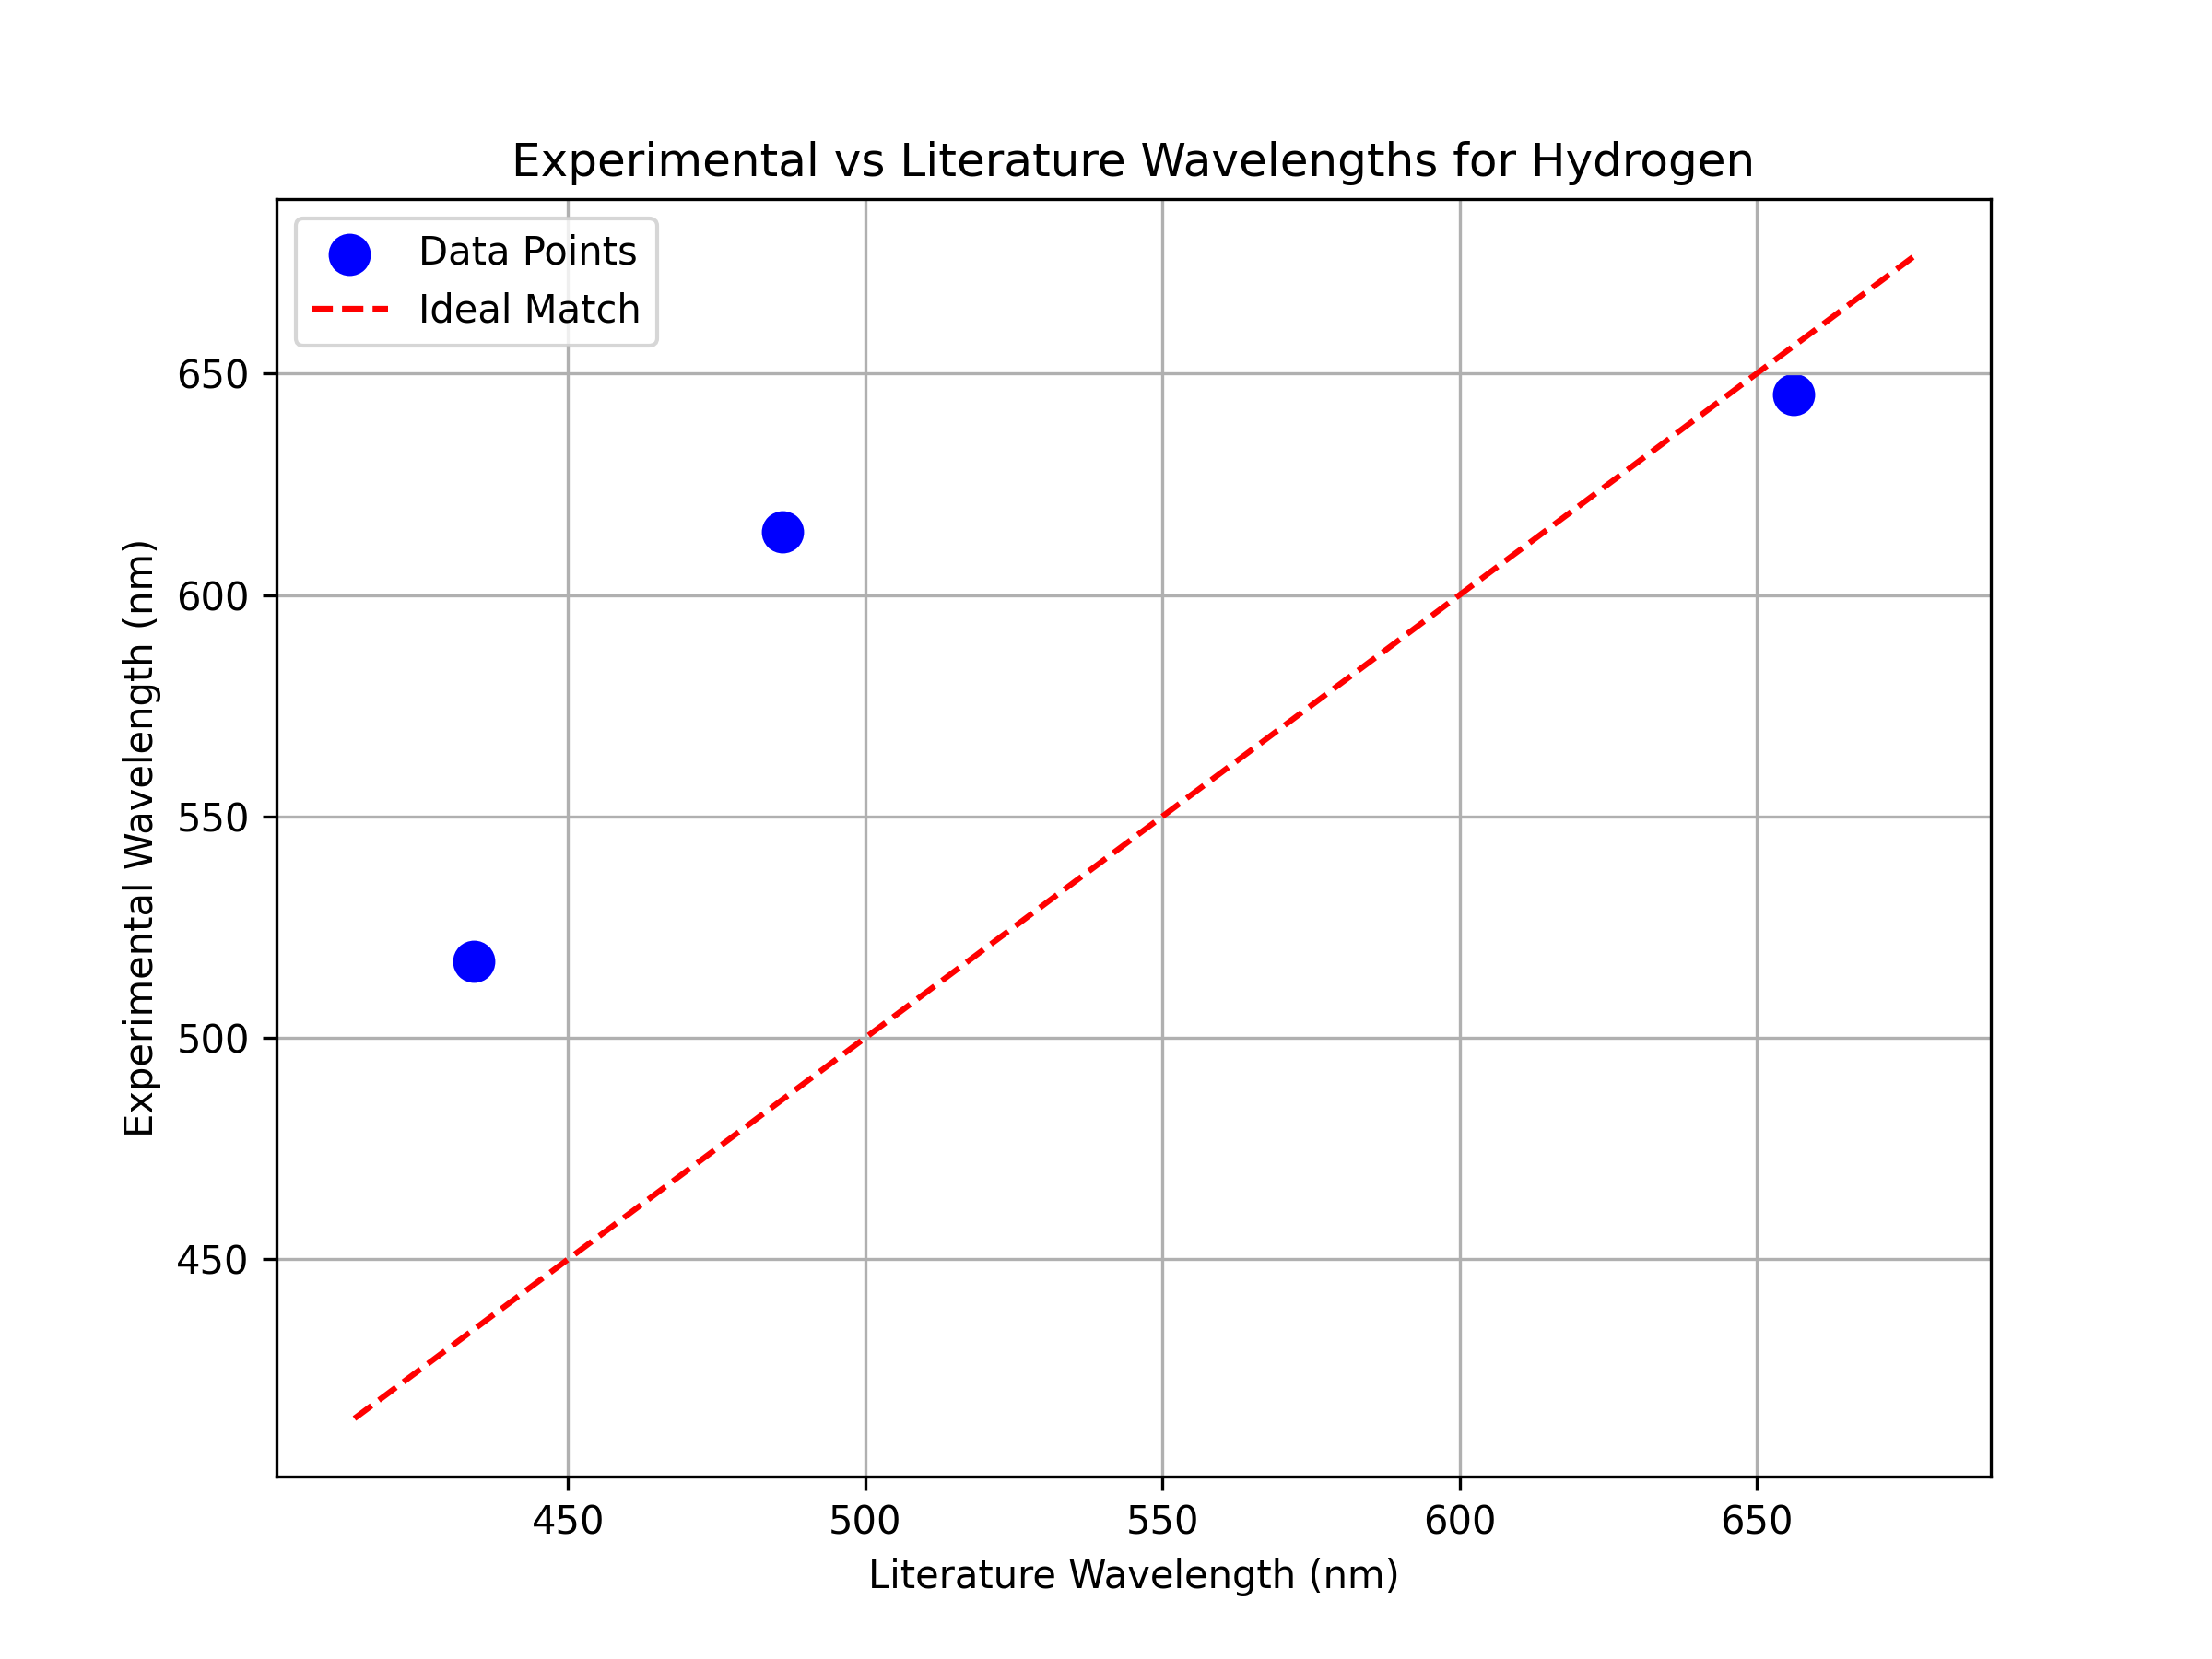
\includegraphics[width=\linewidth]{../plots/wavelength_comparison.png}
    \caption{Experimental vs Literature Wavelengths for the Hydrogen Balmer series. The dashed red line represents the ideal 1:1 match.}
    \label{fig:wavelength}
\end{figure}

% ---------- DISCUSSION ----------
\section{Discussion}
The average experimental Rydberg constant was calculated to be $9.68 \times 10^6\,\mathrm{m^{-1}} \pm 1.31 \times 10^6\,\mathrm{m^{-1}}$. This result is in reasonable agreement with the established literature value of $1.097 \times 10^7\,\mathrm{m^{-1}}$ \cite{lab_manual}. The slight discrepancy is likely due to visual uncertainties when locating the exact spectral lines on the ruler and the alignment of the diffraction grating.

% ---------- INSTRUCTOR'S QUESTIONS ----------
\section{Instructor's Questions}

\textbf{1. Infinite Mass Correction} \\
The difference between using the electron's mass and the reduced mass is very small (about 0.05\%). We can safely ignore this small correction.

\textbf{2. Lifetime of the Excited State} \\
An excited electron is very unstable. It stays in the higher energy level for a very short time, usually about $10^{-8}$ seconds. After that, it quickly drops back down and releases a photon.

\textbf{3. Spontaneous vs. Stimulated Emission} \\
Spontaneous emission happens naturally by itself. However, if an outside photon hits the excited electron and forces it to drop, it is called stimulated emission. So, it can happen with outside help, but the name of the process changes.

\textbf{4. Single vs. Multiple Photon Emission} \\
No, it does not have to be a single photon. The electron can drop directly to the final level (emitting one photon), or it can drop step-by-step. If it drops step-by-step, it emits multiple photons with lower energies.

% ---------- CONCLUSION ----------
\section{Conclusion}
The atomic spectra of hydrogen were successfully observed, and the wavelengths of the first three lines of the Balmer series were measured. Using the grating equation, the wavelengths were calculated, which in turn allowed for the experimental determination of the Rydberg constant. The results demonstrate the discrete nature of atomic energy transitions as described by the Bohr model, and the derived Rydberg constant is in general agreement with the literature value, validating the theoretical framework.

% ---------- ADDITIONAL RESOURCES ----------
\section{Additional Resources}
Source code and related materials for the experiments are available on GitHub.

\begin{figure}[H]
    \centering
    \begin{minipage}{0.15\textwidth}
        \centering
        \qrcode[height=1.5cm]{https://github.com/ibeuler/LAB-Reports.git}
    \end{minipage}%
    \begin{minipage}{0.2\textwidth}
        \raggedright
        \caption{Access the GitHub repository for source code and related experiments.}
        \label{fig:qr_code}
    \end{minipage}
\end{figure}

\begin{thebibliography}{9}
\bibitem{lab_manual}
    ISTANBUL UNIVERSITY, \textit{ATOMIC AND MOLECULAR PHYSICS LABORATORY EXPERIMENTS MANUAL}, Department of Physics.
\bibitem{haken_wolf}
    H Haken, H C Wolf, \textit{The Physics of Atoms and Quanta}, 2000, Springer.
\end{thebibliography}

\end{document}
